\subsubsection{Đăng ký, đăng nhập và quản lý hồ sơ}
\label{sec:screen-account}
Biểu mẫu tài khoản kiểm tra thông tin bắt buộc, email, số điện thoại và mật khẩu trước khi gửi. AuthViewModel giữ trạng thái xử lý; FirebaseAuthRepository xác thực bằng email hoặc tra cứu username trong \texttt{usernames}. UID đăng nhập liên kết với hồ sơ \texttt{users}; vai trò và trạng thái quyết định khu vực được mở, không lấy trực tiếp từ dữ liệu người dùng tự nhập \parencite{broomsharing_source}.

Hình~\ref{fig:actual-account} minh họa màn đăng nhập và hồ sơ hiện thực. Chức năng quên mật khẩu gửi liên kết qua Firebase Authentication. Hồ sơ cho phép chọn ảnh từ thư viện hoặc nhập URL; ảnh được kiểm tra, tải lên Cloudinary rồi cập nhật \texttt{photoUrl}. Với Host, ảnh và bản chiếu \texttt{publicHosts} được đồng bộ trong transaction. Ảnh hồ sơ được tải bằng Picasso; cập nhật ảnh không cho phép sửa vai trò hoặc trạng thái tài khoản.

\begin{figure}[H]\centering
\begin{minipage}[t]{0.34\linewidth}\centering
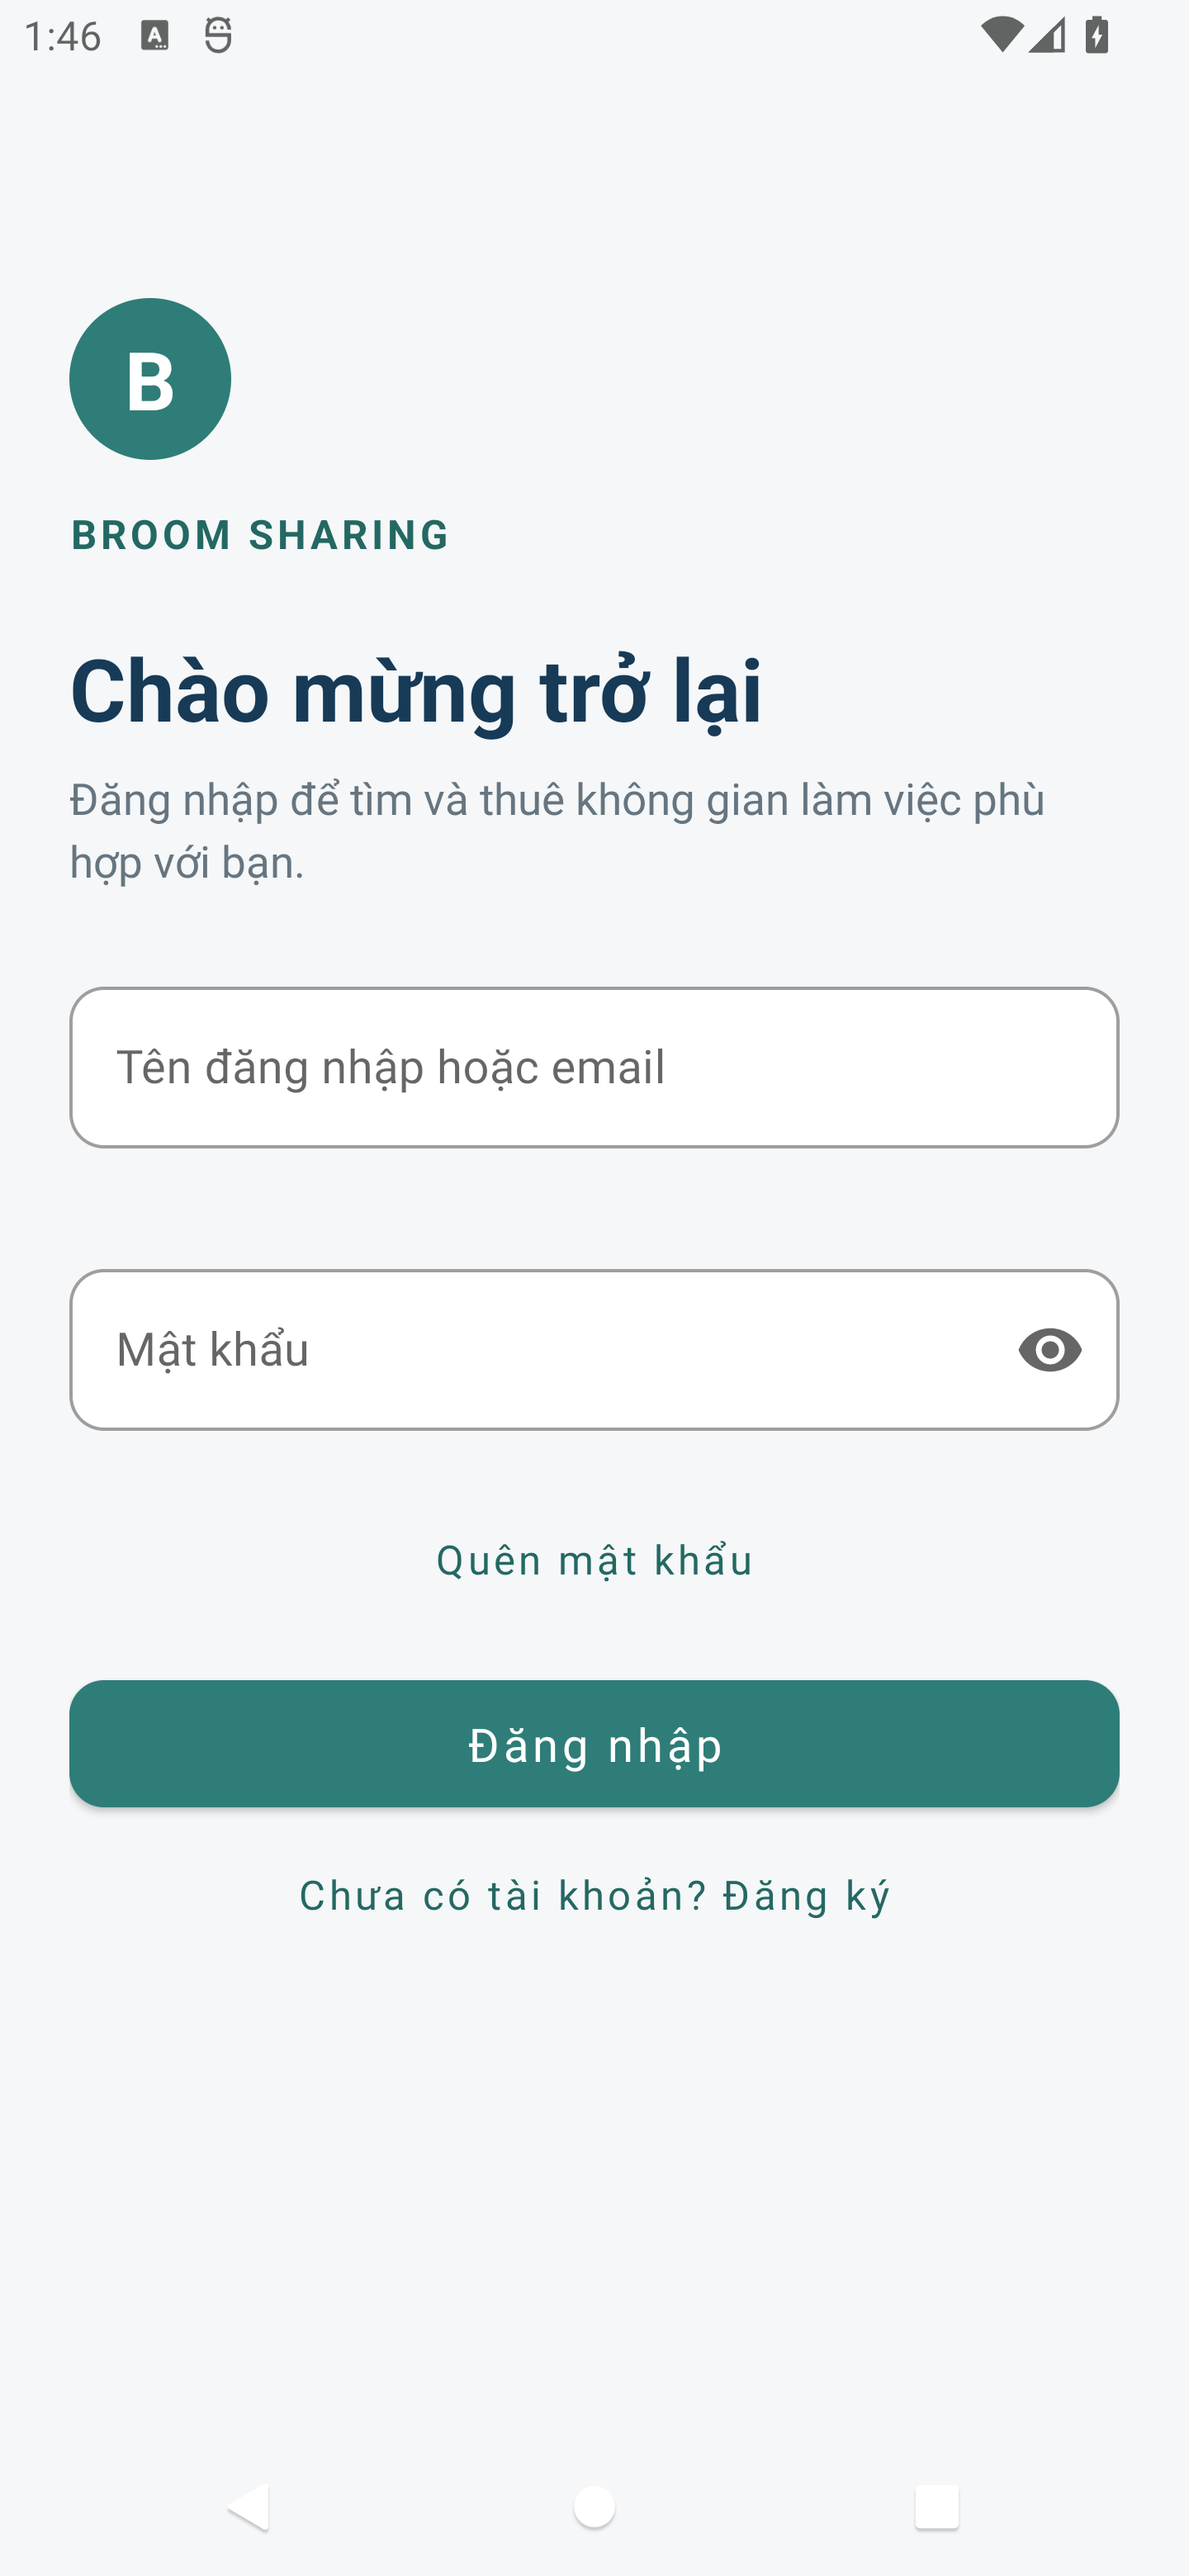
\includegraphics[width=\linewidth]{chapter5/final/login.png}\\[-1mm]
{\small (a) Đăng nhập}
\end{minipage}\hspace{0.05\linewidth}%
\begin{minipage}[t]{0.34\linewidth}\centering
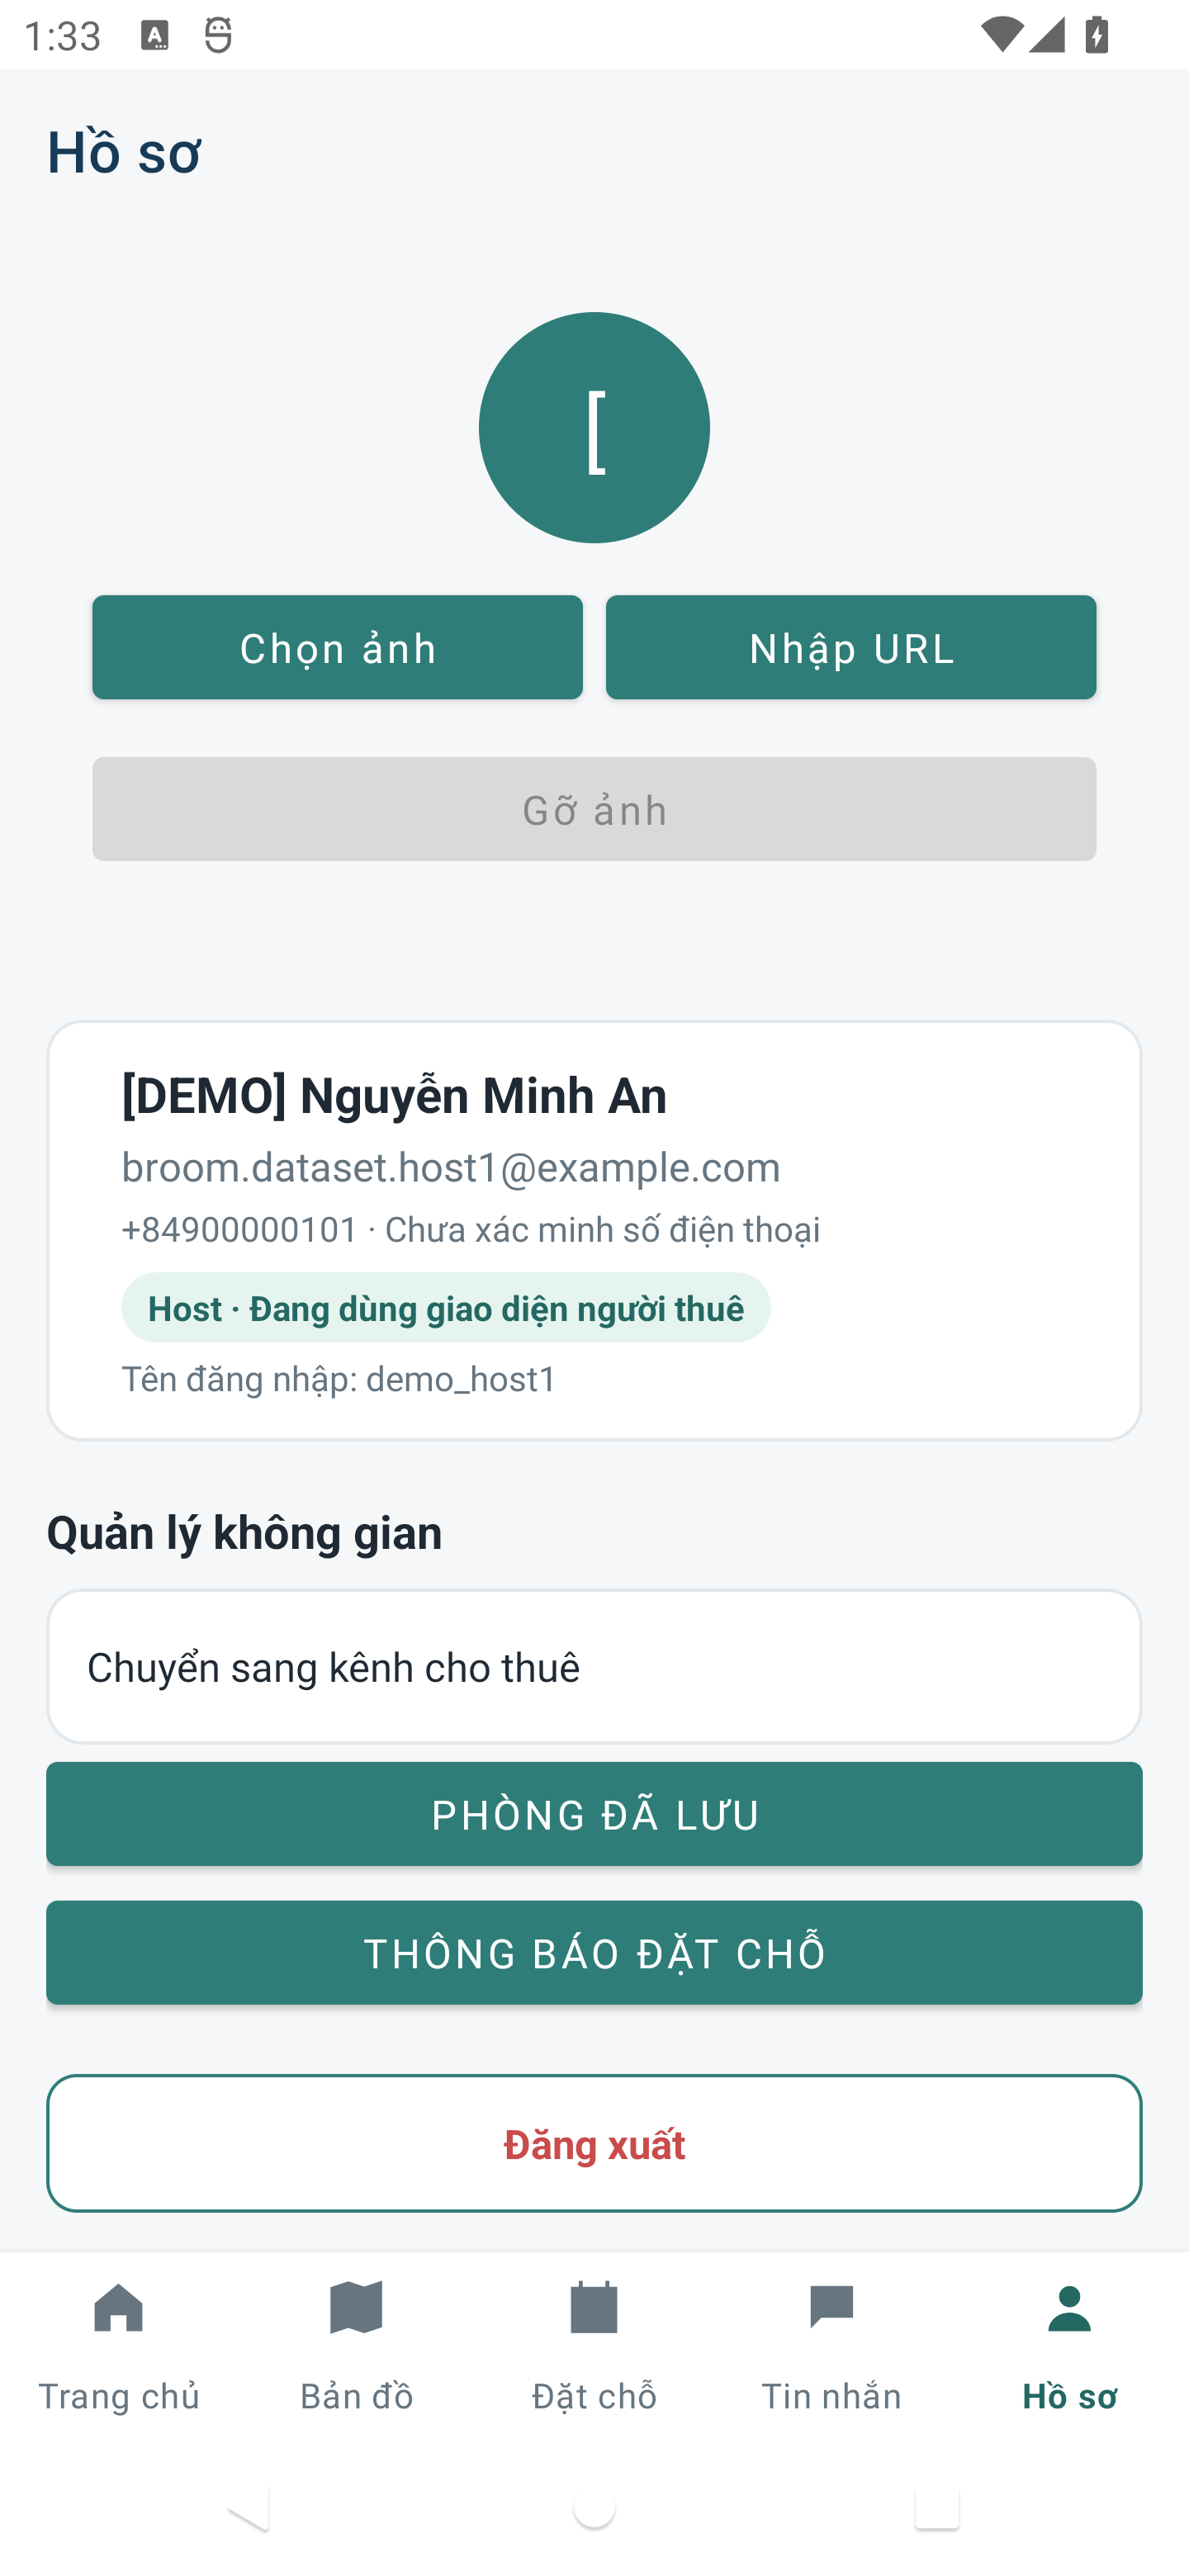
\includegraphics[width=\linewidth]{chapter5/final/profile.png}\\[-1mm]
{\small (b) Hồ sơ và ảnh đại diện}
\end{minipage}
\caption{Giao diện xác thực và hồ sơ tài khoản}
\label{fig:actual-account}
\end{figure}

\subsubsection{Trang chủ, tìm kiếm và chi tiết không gian}
\label{sec:screen-discovery}
Trang chủ tải phòng đã duyệt, đang hoạt động theo từng trang 20 document. RoomRepository bổ sung thông tin Building và PublicHost để tạo RoomListing; RoomViewModel ghép theo Room ID và giữ con trỏ tải tiếp. Từ khóa và bộ lọc khu vực, loại phòng, chế độ thuê, sức chứa, giá được áp dụng trên dữ liệu đã tải; khi cần, ứng dụng tải tiếp trước khi kết luận không có kết quả.

Hình~\ref{fig:actual-discovery} cho thấy thẻ phòng và trang chi tiết cùng đối tượng. Chi tiết hiển thị ảnh, đơn vị giá, tiện ích, lịch hoạt động và chính sách; các nút lưu, liên hệ và đặt chỗ giữ nguyên Room ID. FavoritesRepository ghi hoặc xóa document \texttt{users/\{uid\}/favorites/\{roomId\}}. Với phòng tháng/quý, nhãn lịch được dựng từ lịch tháng, phân biệt kỳ trống, tạm giữ, đặt trước và kỳ thuê còn tối đa ba ngày; nhãn không thay cho bước kiểm tra kỳ thuê cụ thể.

\begin{figure}[H]\centering
\begin{minipage}[t]{0.34\linewidth}\centering
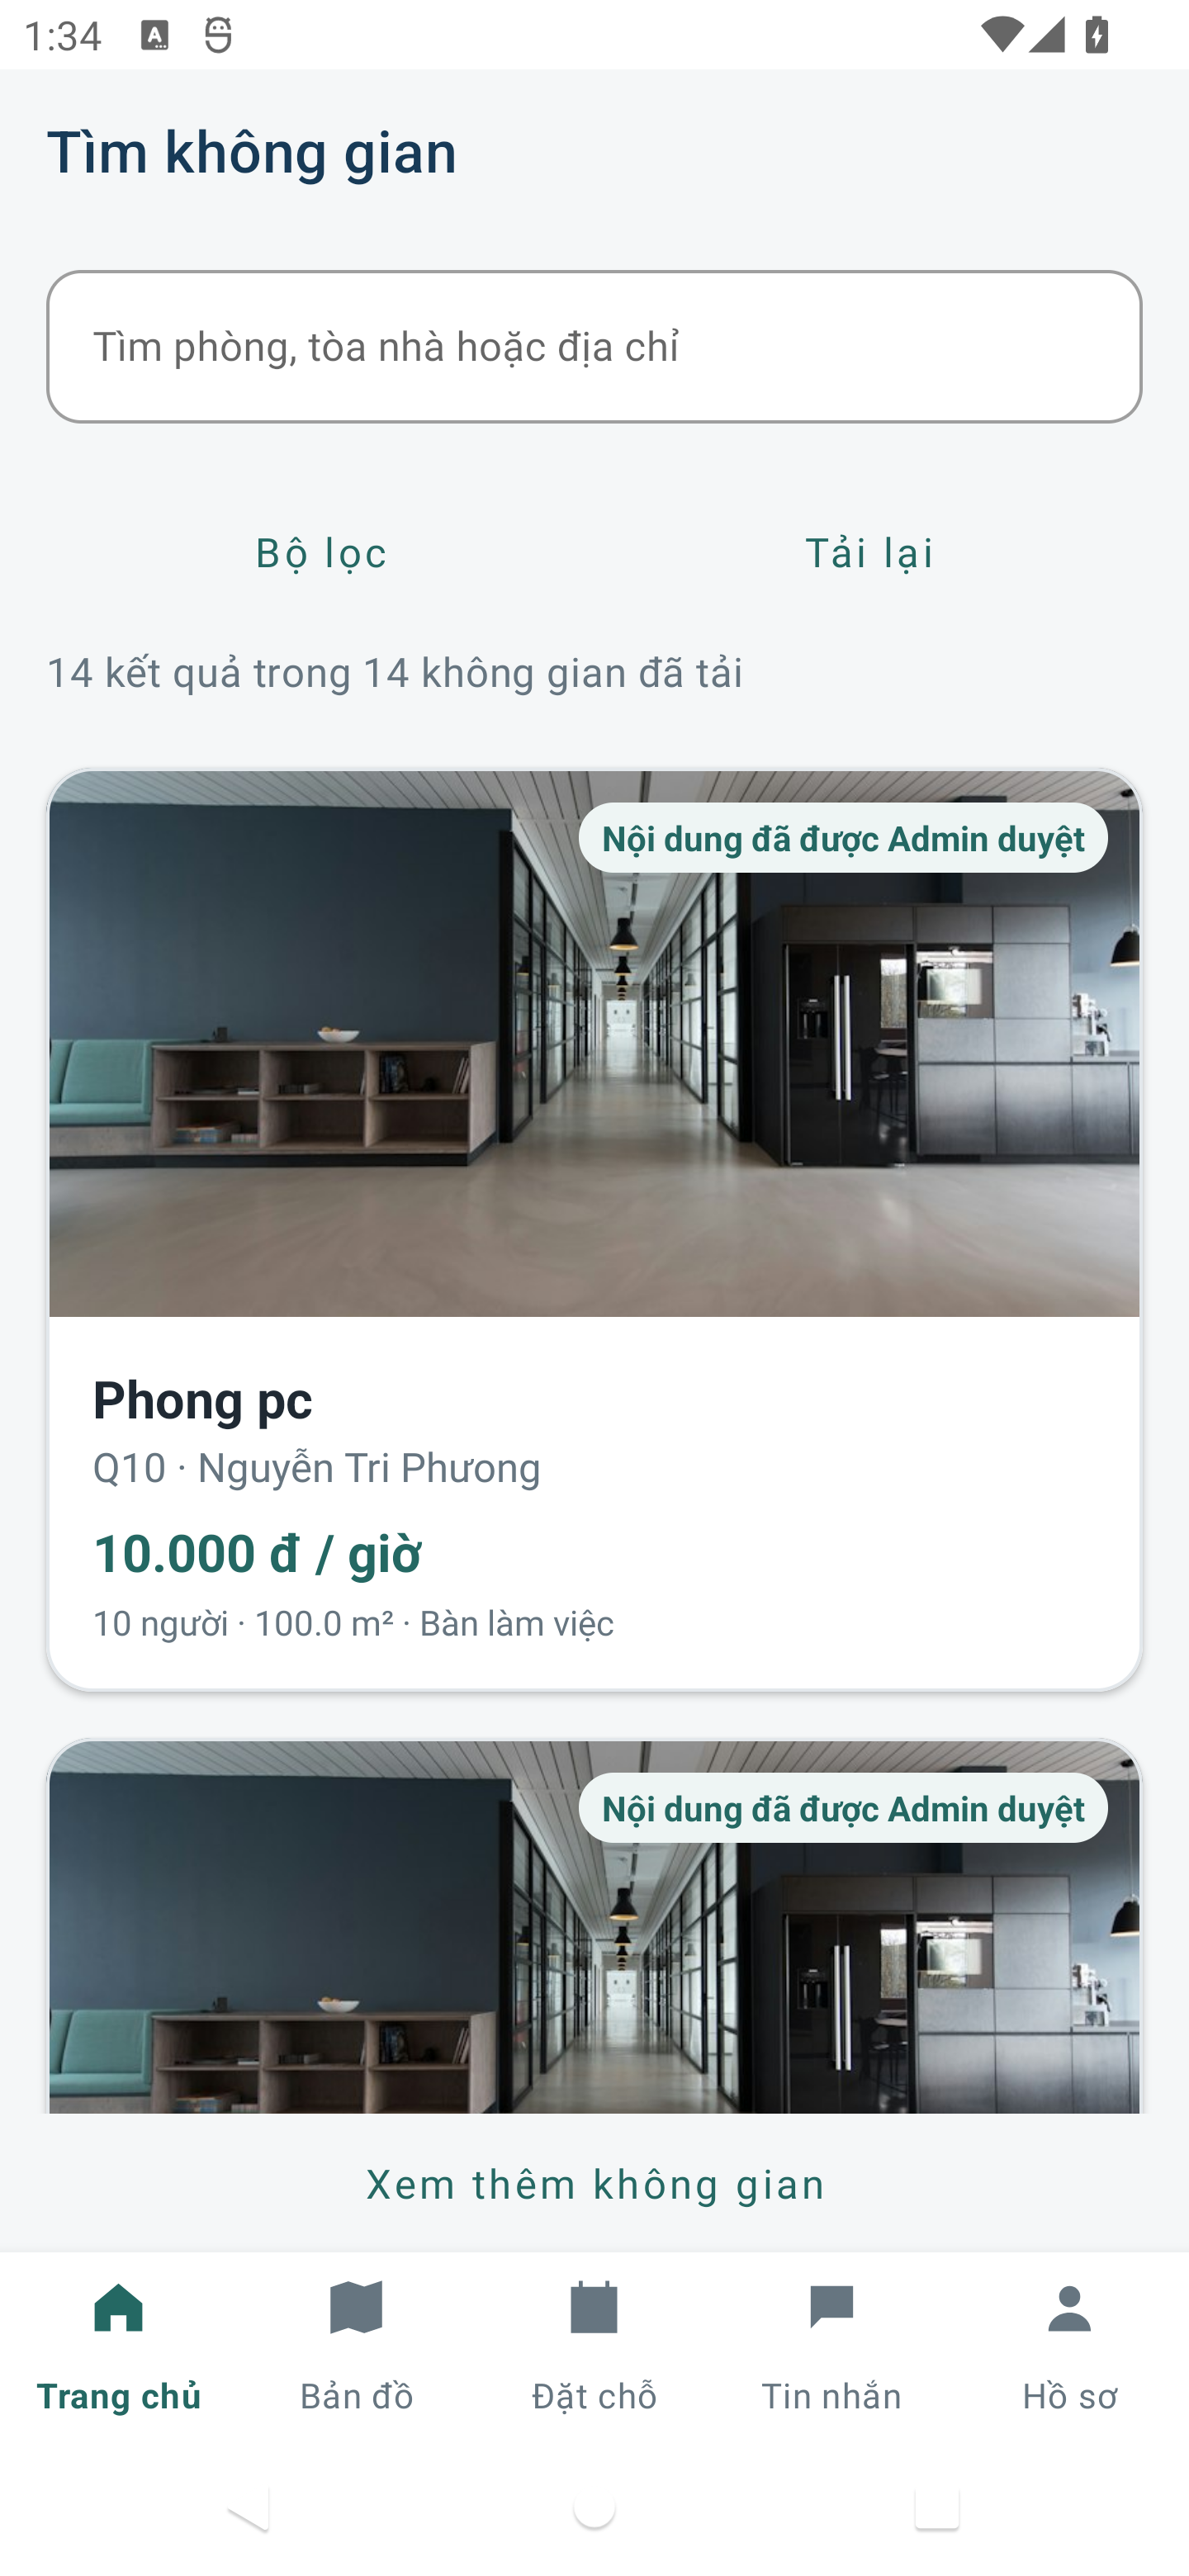
\includegraphics[width=\linewidth]{chapter5/final/home.png}\\[-1mm]
{\small (a) Danh sách phòng}
\end{minipage}\hspace{0.05\linewidth}%
\begin{minipage}[t]{0.34\linewidth}\centering
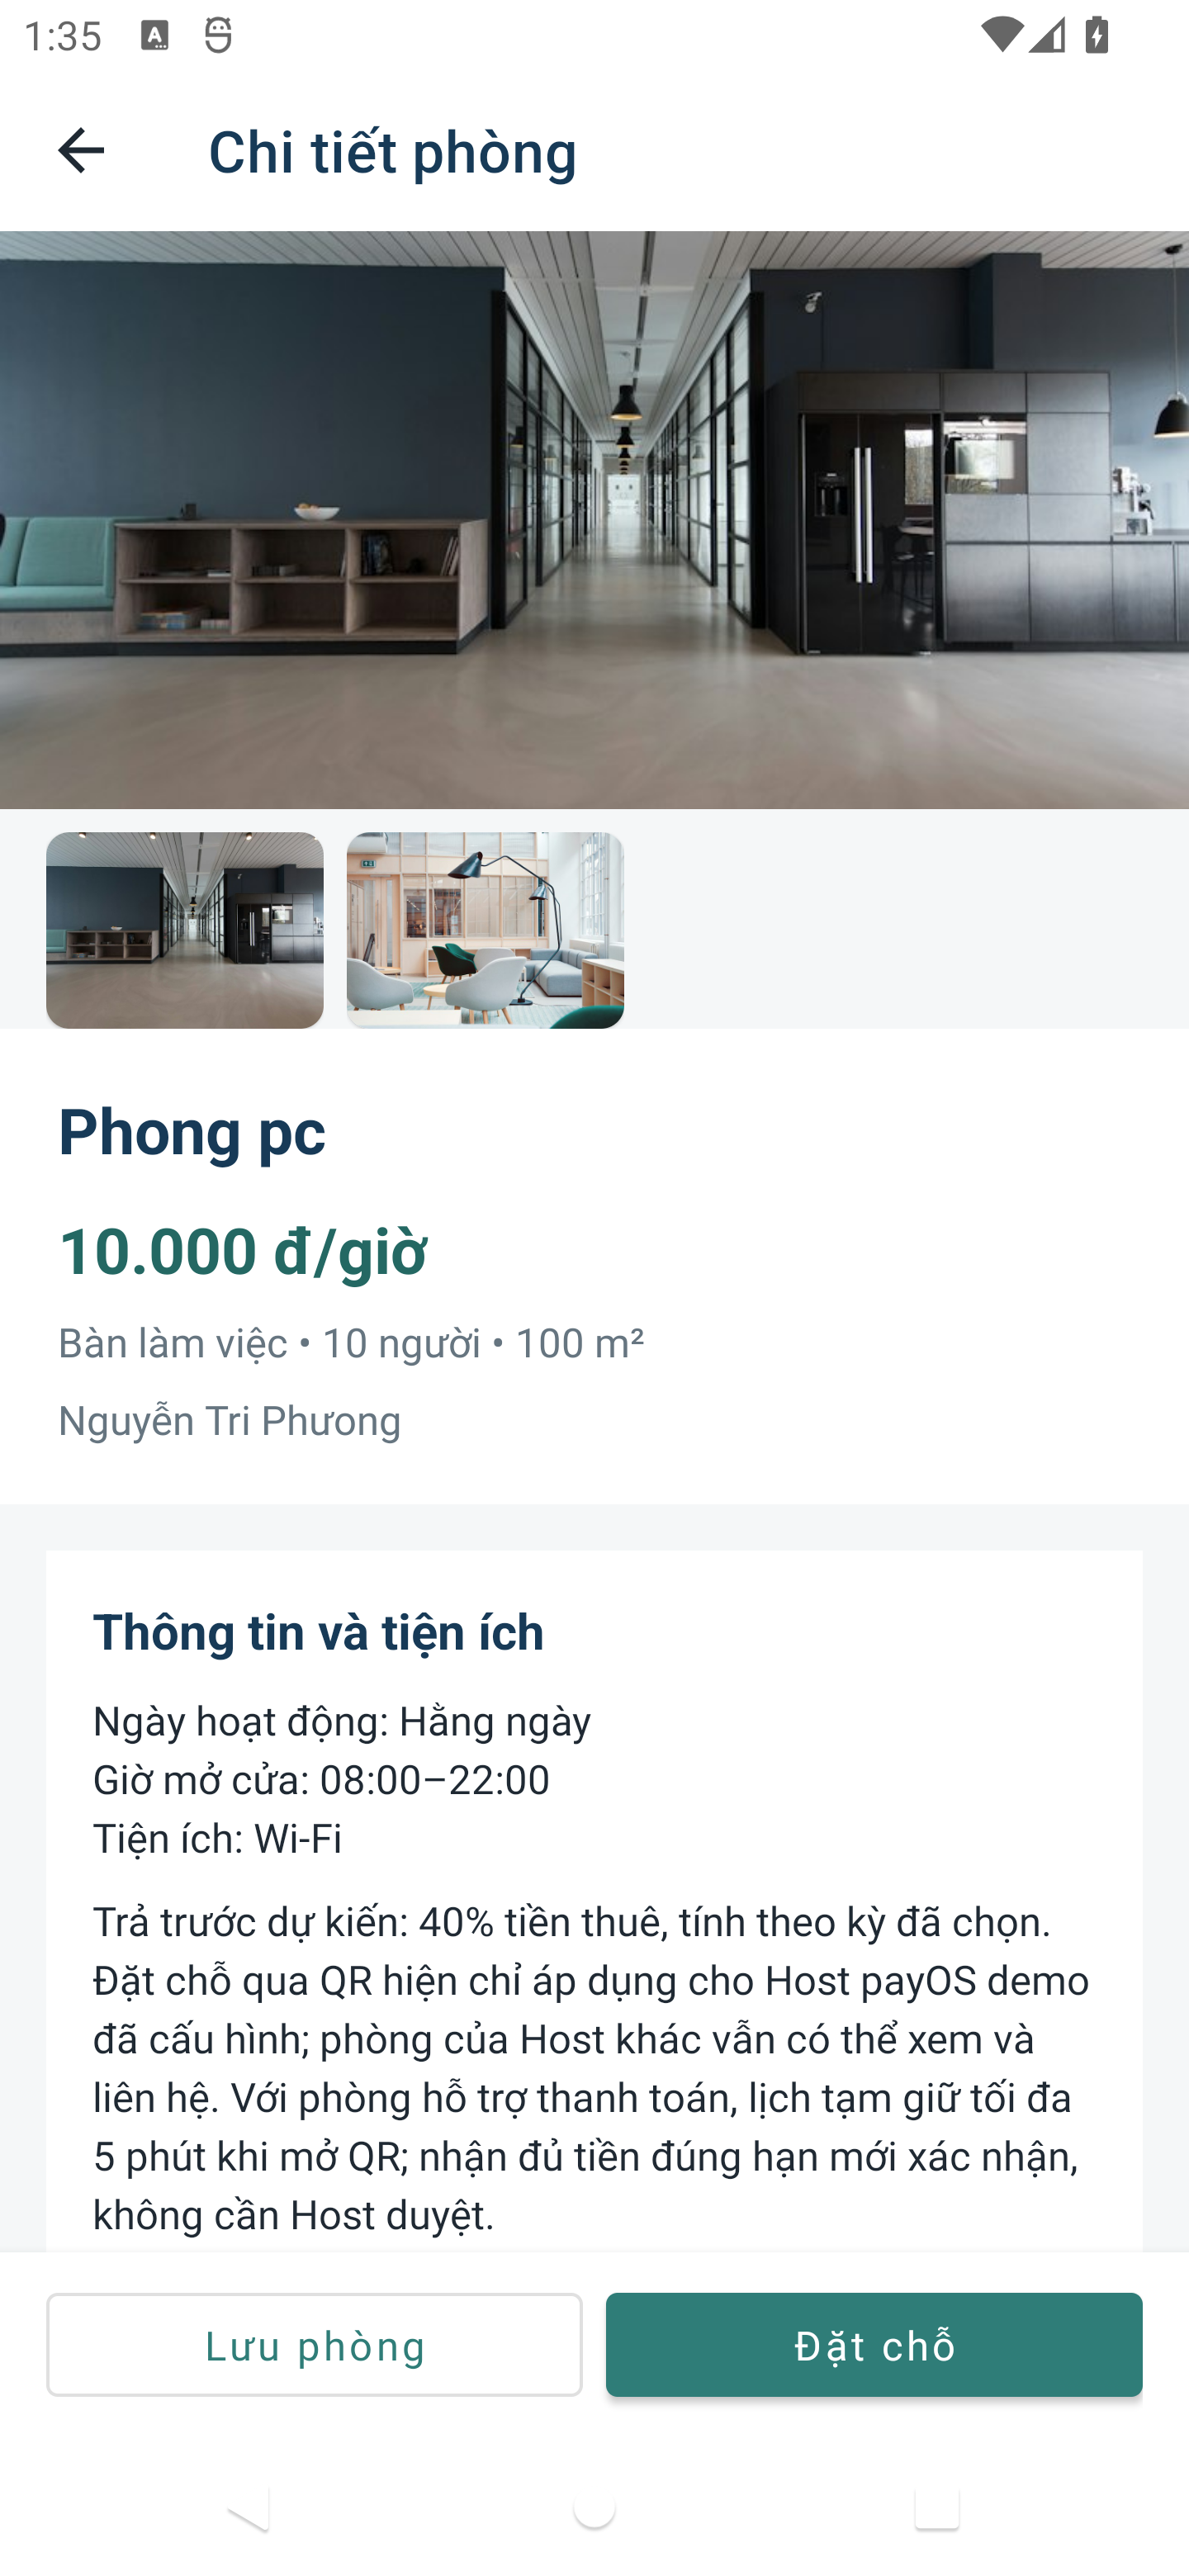
\includegraphics[width=\linewidth]{chapter5/final/detail.png}\\[-1mm]
{\small (b) Chi tiết phòng}
\end{minipage}
\caption{Từ danh sách không gian đến thông tin chi tiết}
\label{fig:actual-discovery}
\end{figure}

\subsubsection{Bản đồ và tìm đường}
\label{sec:screen-map}
Màn bản đồ kết hợp phòng từ Firestore với tọa độ tòa nhà, vị trí thiết bị hoặc tâm tìm kiếm do người dùng chọn. MapLibre Native dựng nền bản đồ từ MapTiler; MapRepository xử lý geocoding và tuyến ô tô từ openrouteservice. Khoảng cách dùng lọc lân cận được tính tại ứng dụng, chưa có truy vấn bán kính bằng geohash trên Firestore.

Hình~\ref{fig:actual-map} thể hiện điểm đến, tuyến đường và nút Xem phòng trên tablet. Nút này mở đúng chi tiết theo Room ID để tiếp tục đặt thuê. Địa điểm tham khảo được phân biệt với phòng trong app và dẫn tới nguồn tin; chúng chưa có chức năng đặt chỗ. Thời gian di chuyển là ước tính của tuyến, không bao gồm tình trạng giao thông trực tiếp.

\begin{figure}[H]\centering
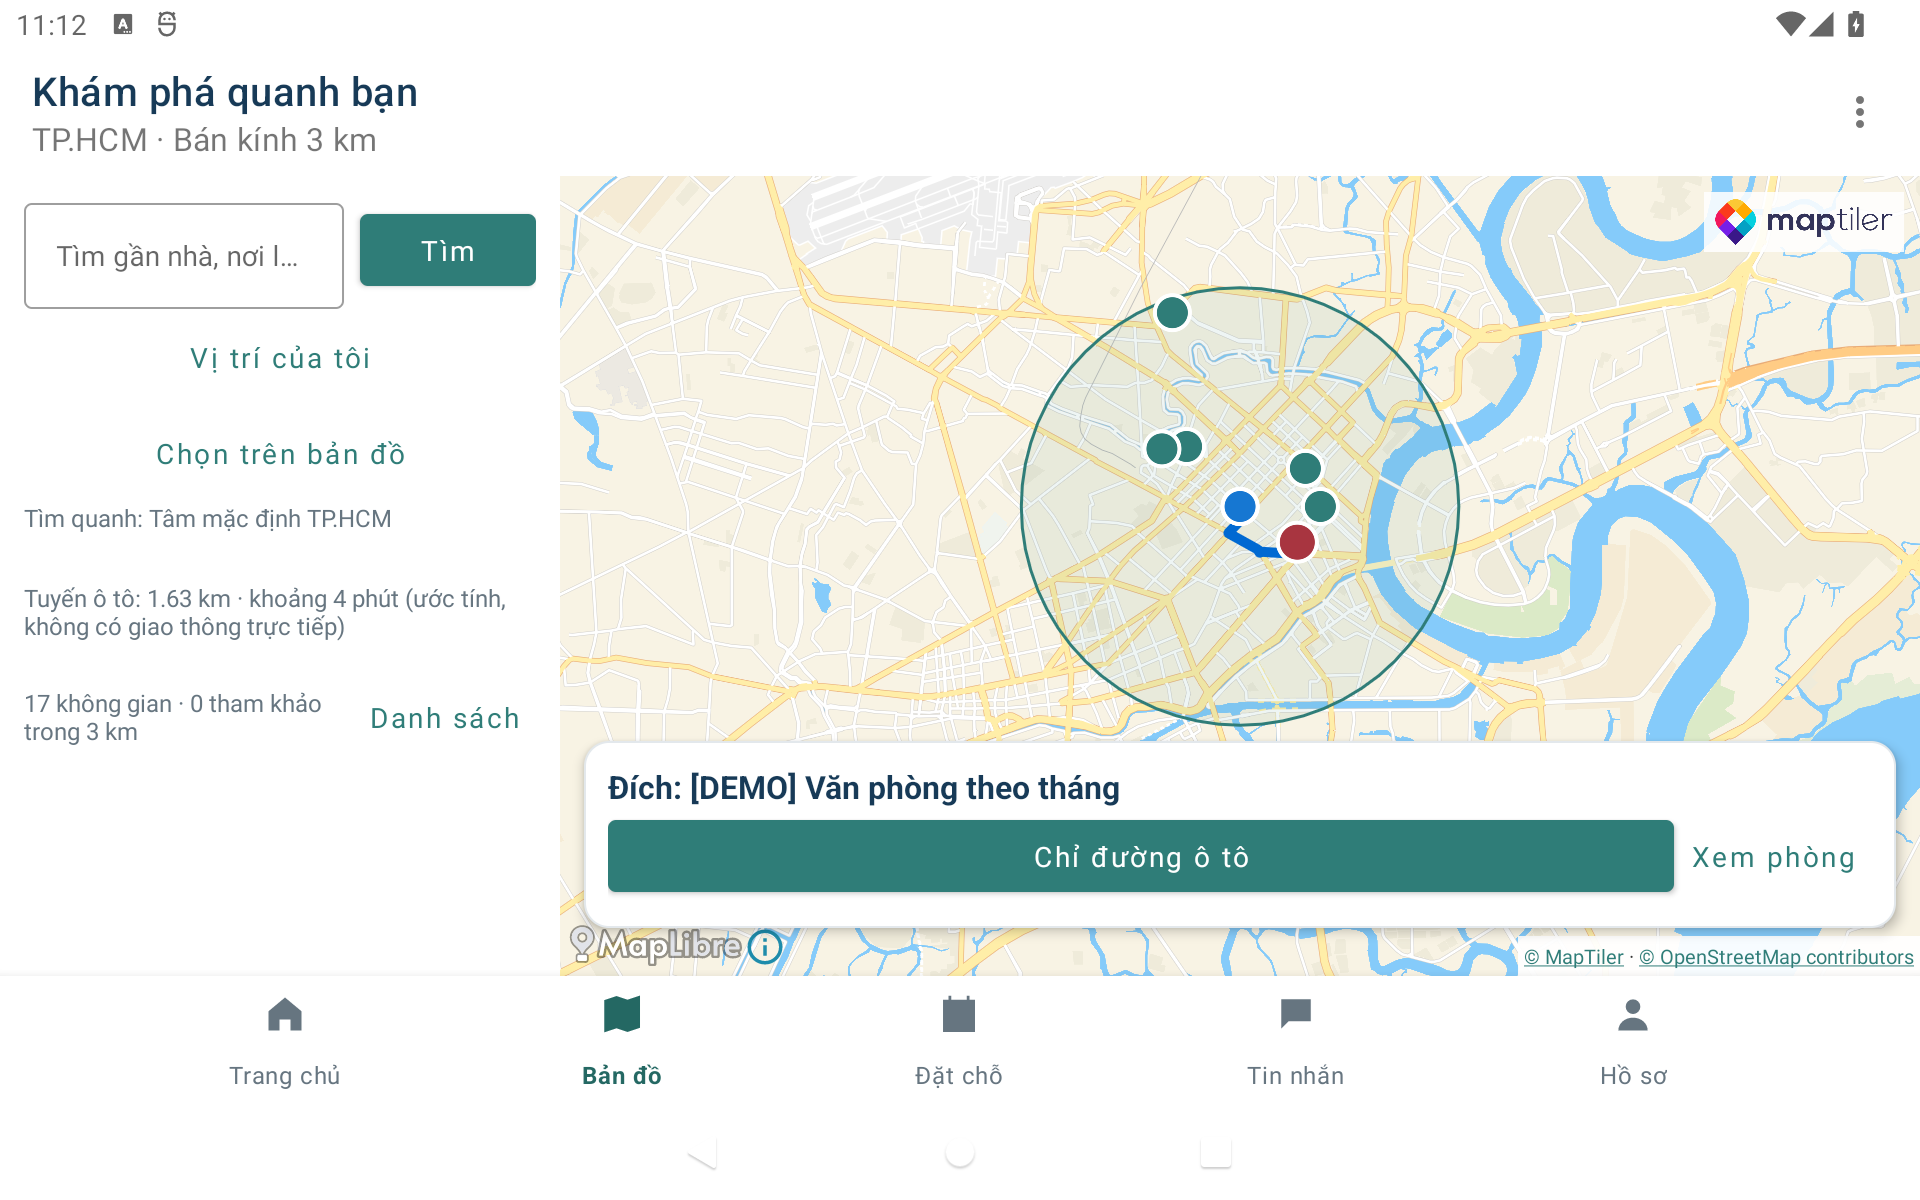
\includegraphics[width=0.96\linewidth]{chapter5/members/user-tablet-map-selected-landscape.png}
\caption{Chọn điểm đến, tìm đường và mở phòng từ bản đồ}
\label{fig:actual-map}
\end{figure}

\subsubsection{Đặt chỗ và thanh toán}
\label{sec:screen-payment}
BookingActivity hiển thị bộ chọn thời gian theo hình thức thuê của phòng. Sau khi kiểm tra lịch và giá, nút thanh toán tạo booking PENDING cùng khóa lịch tạm trong transaction và mở QR ngay. Thời hạn tối đa năm phút, không vượt giờ bắt đầu; mở lại phiên không gia hạn. Luồng mới không cần Host duyệt.

PaymentRepository gửi booking ID và ID token tới backend Java. Backend xác thực kênh Host demo, lấy khoản trả trước 40\% từ giá đã chốt và tạo giao dịch payOS. Đủ tiền đúng hạn mới cập nhật PAID/CONFIRMED; hết hạn chưa trả dẫn tới kết quả không thành công và nhả lịch sau đối soát. Listener cập nhật màn QR, thẻ tiếp tục thanh toán và thông báo điện thoại. Các màn và kết quả tương ứng được thể hiện tại Mục~\ref{sec:execution-booking-payment}. QR dùng cho thanh toán; Host ghi nhận việc nhận phòng bằng thao tác riêng.

\subsubsection{Quản lý lượt thuê, đánh giá và báo cáo}
\label{sec:screen-rentals}
MyBookingsActivity theo dõi booking theo UID người thuê, sắp thời điểm tạo giảm dần và lọc trạng thái trên giao diện. Trang chi tiết chỉ mở các thao tác còn hợp lệ; trước khi hủy, Repository kiểm tra lại người thực hiện, thời gian và trạng thái. Lịch sử được giữ sau khi khép lượt, đồng thời tách trạng thái tiền khỏi trạng thái sử dụng.

Hình~\ref{fig:actual-rentals} minh họa booking hết hạn chưa thanh toán trên tablet. Đánh giá chỉ được gửi cho lượt đã khép, có xác nhận sử dụng; ReviewRepository ghi một document \texttt{reviews/\{bookingId\}} cho mỗi booking, gồm điểm tổng quan và nhận xét. Báo cáo vi phạm ghi vào \texttt{reports}; người gửi theo dõi kết quả, Host phản hồi hồ sơ còn mở và Admin kết luận. Chức năng lưu lịch mở biểu mẫu của ứng dụng Lịch bằng Intent; người dùng xác nhận việc lưu và lịch thiết bị không tự đổi khi booking bị hủy.

\begin{figure}[H]\centering
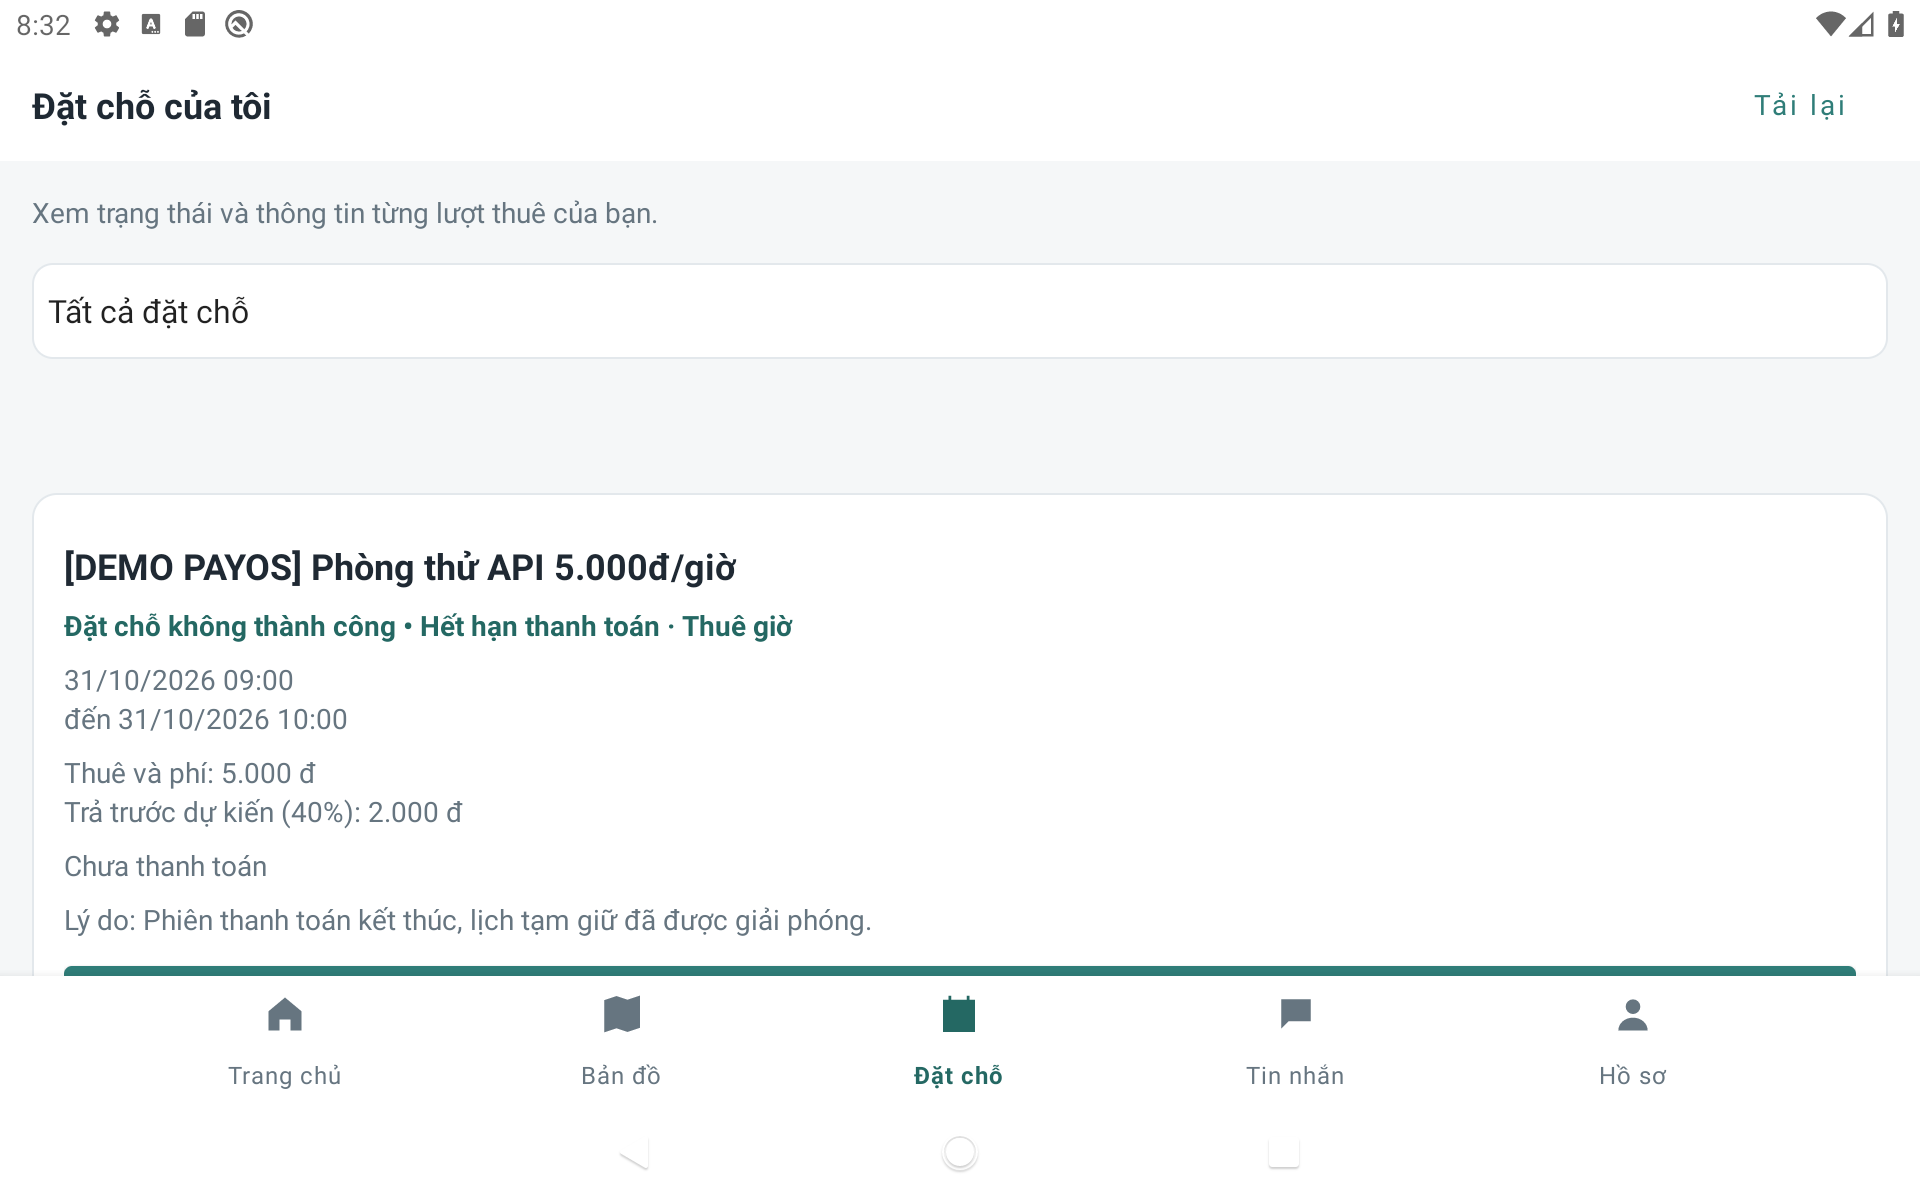
\includegraphics[width=0.96\linewidth]{chapter5/members/user-tablet-bookings-landscape.png}
\caption{Danh sách lượt thuê và kết quả hết hạn thanh toán}
\label{fig:actual-rentals}
\end{figure}

\subsubsection{Tin nhắn và thông báo}
\label{sec:screen-messages}
Inbox truy vấn \texttt{conversations} theo \texttt{memberUids}; mỗi hội thoại có subcollection \texttt{messages}, sắp bằng \texttt{sequence} và giới hạn số tin tải. Transaction gửi tin ghi message, preview, thứ tự và bộ đếm nhận; mốc đọc chỉ tăng cho bên đang đọc. Conversation ID theo cặp người thuê và Host cho phép tiếp tục trao đổi mà không tạo một hội thoại mới cho mỗi lần mở phòng.

Hình~\ref{fig:actual-messages} thể hiện danh sách hội thoại và màn trao đổi với Host của phòng PAYOS. Hội thoại mới hiển thị phòng ngữ cảnh và ô gửi tin trước khi có nội dung trao đổi. Hộp cập nhật tổng hợp sự kiện booking, hội thoại và báo cáo, còn \texttt{noticeReads} chỉ lưu mốc đã đọc. PaymentReminderService hiển thị phiên còn hạn và đổi thông báo theo kết quả, như Hình~\ref{fig:booking-resume-notification}; quyền thông báo không quyết định trạng thái thanh toán trên server.

\begin{figure}[H]\centering
\begin{minipage}[t]{0.34\linewidth}\centering
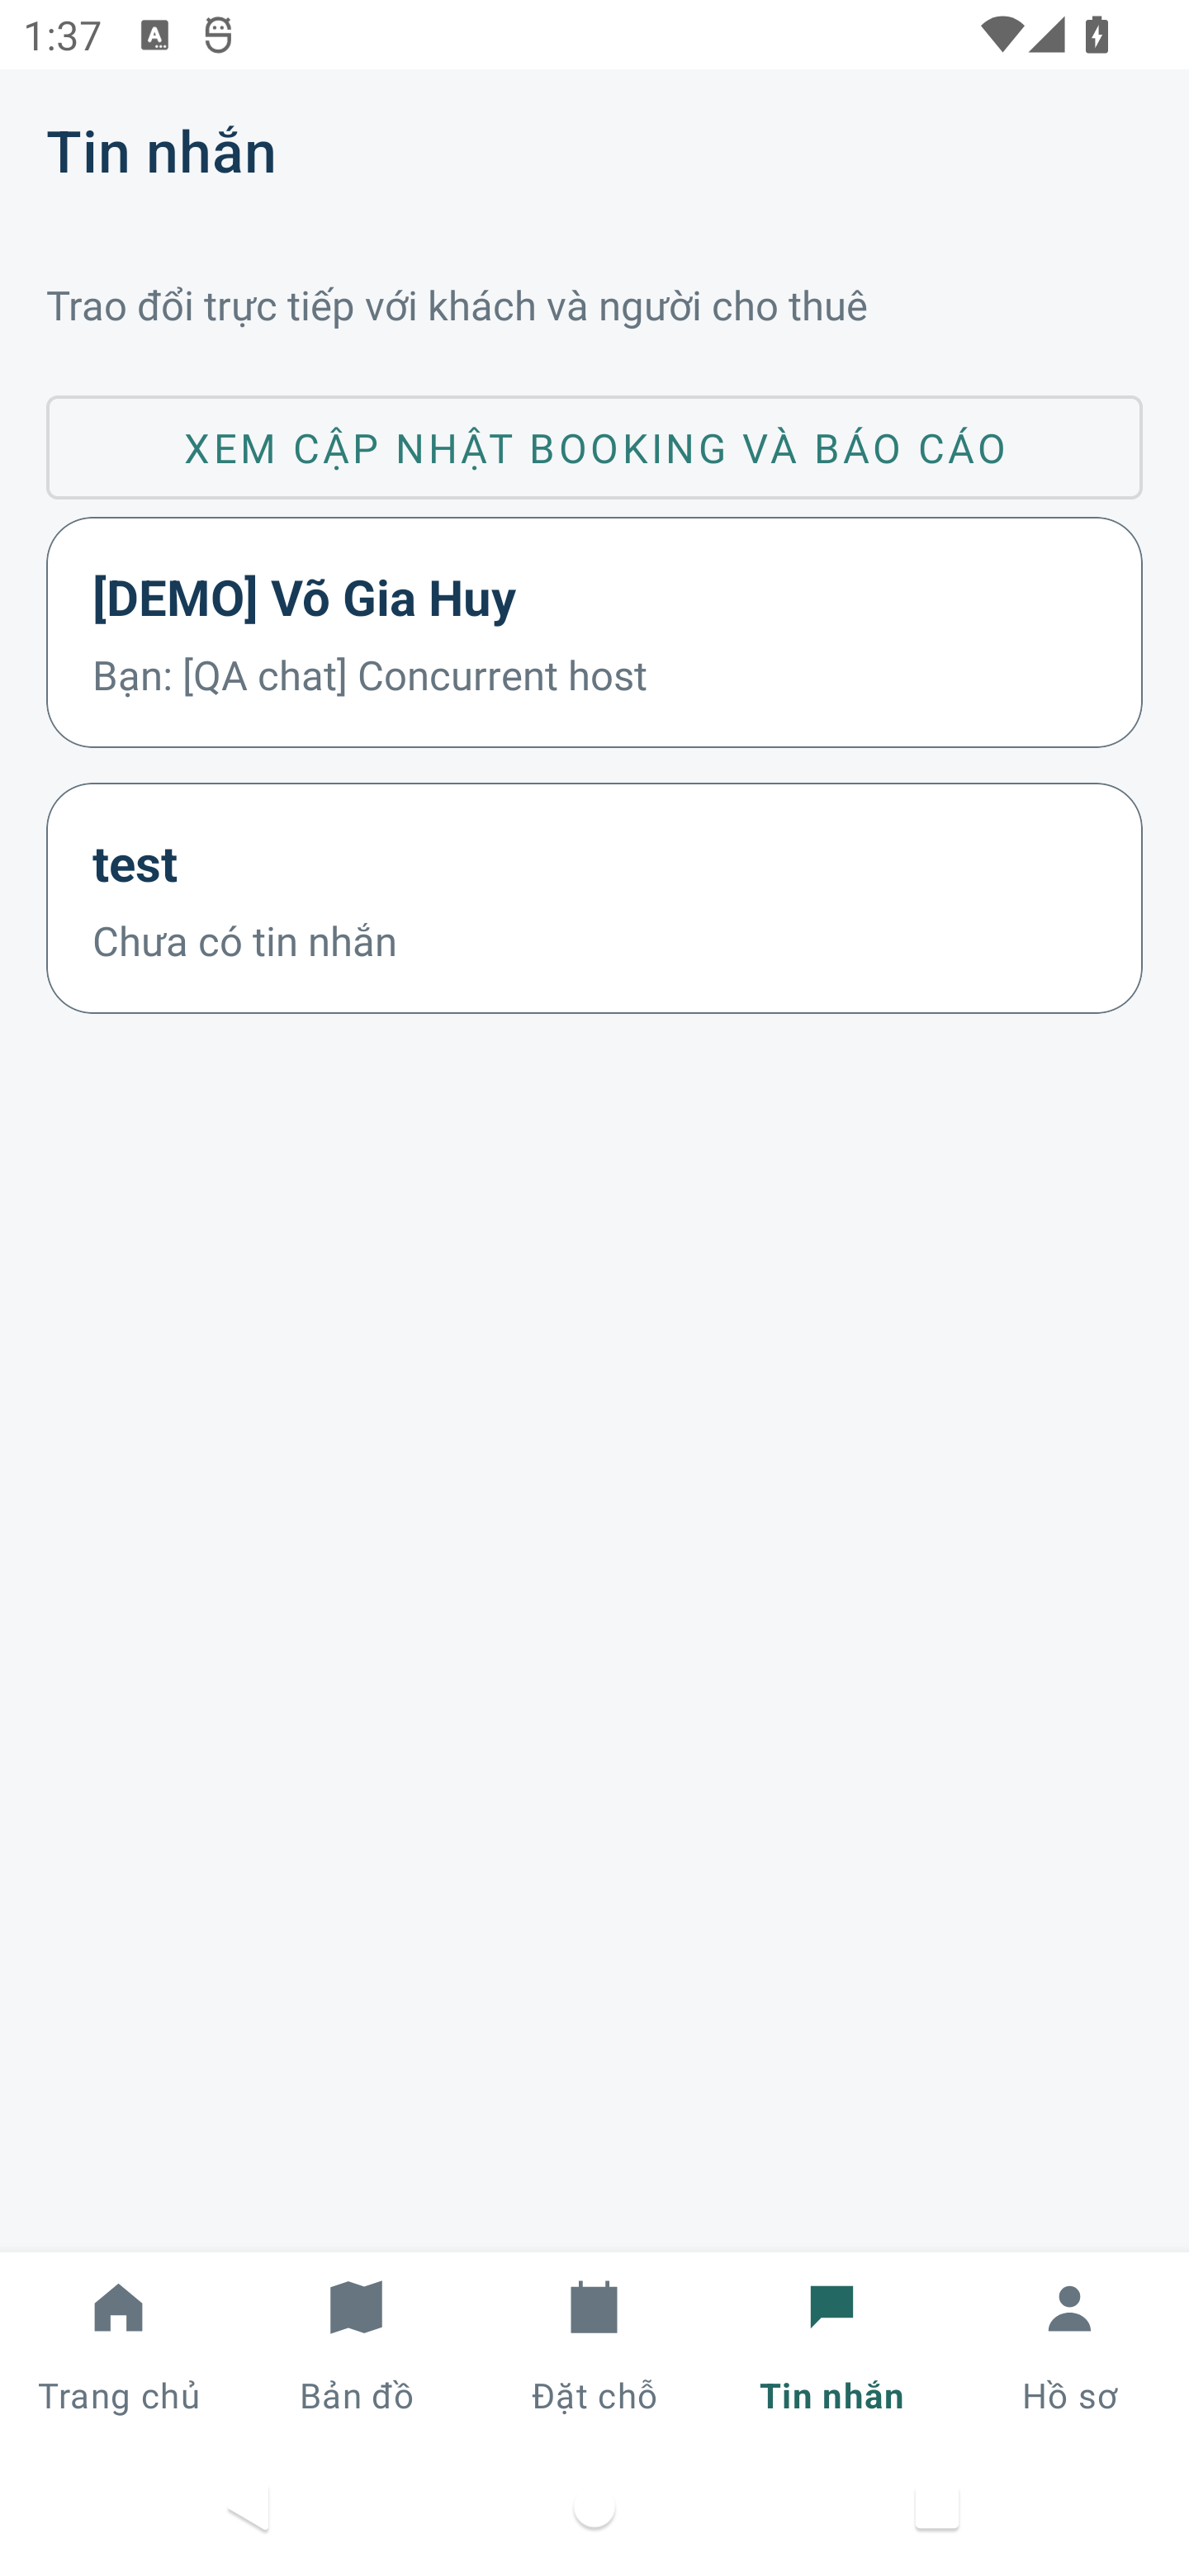
\includegraphics[width=\linewidth]{chapter5/final/conversations.png}\\[-1mm]
{\small (a) Danh sách hội thoại DEMO}
\end{minipage}\hspace{0.05\linewidth}%
\begin{minipage}[t]{0.34\linewidth}\centering
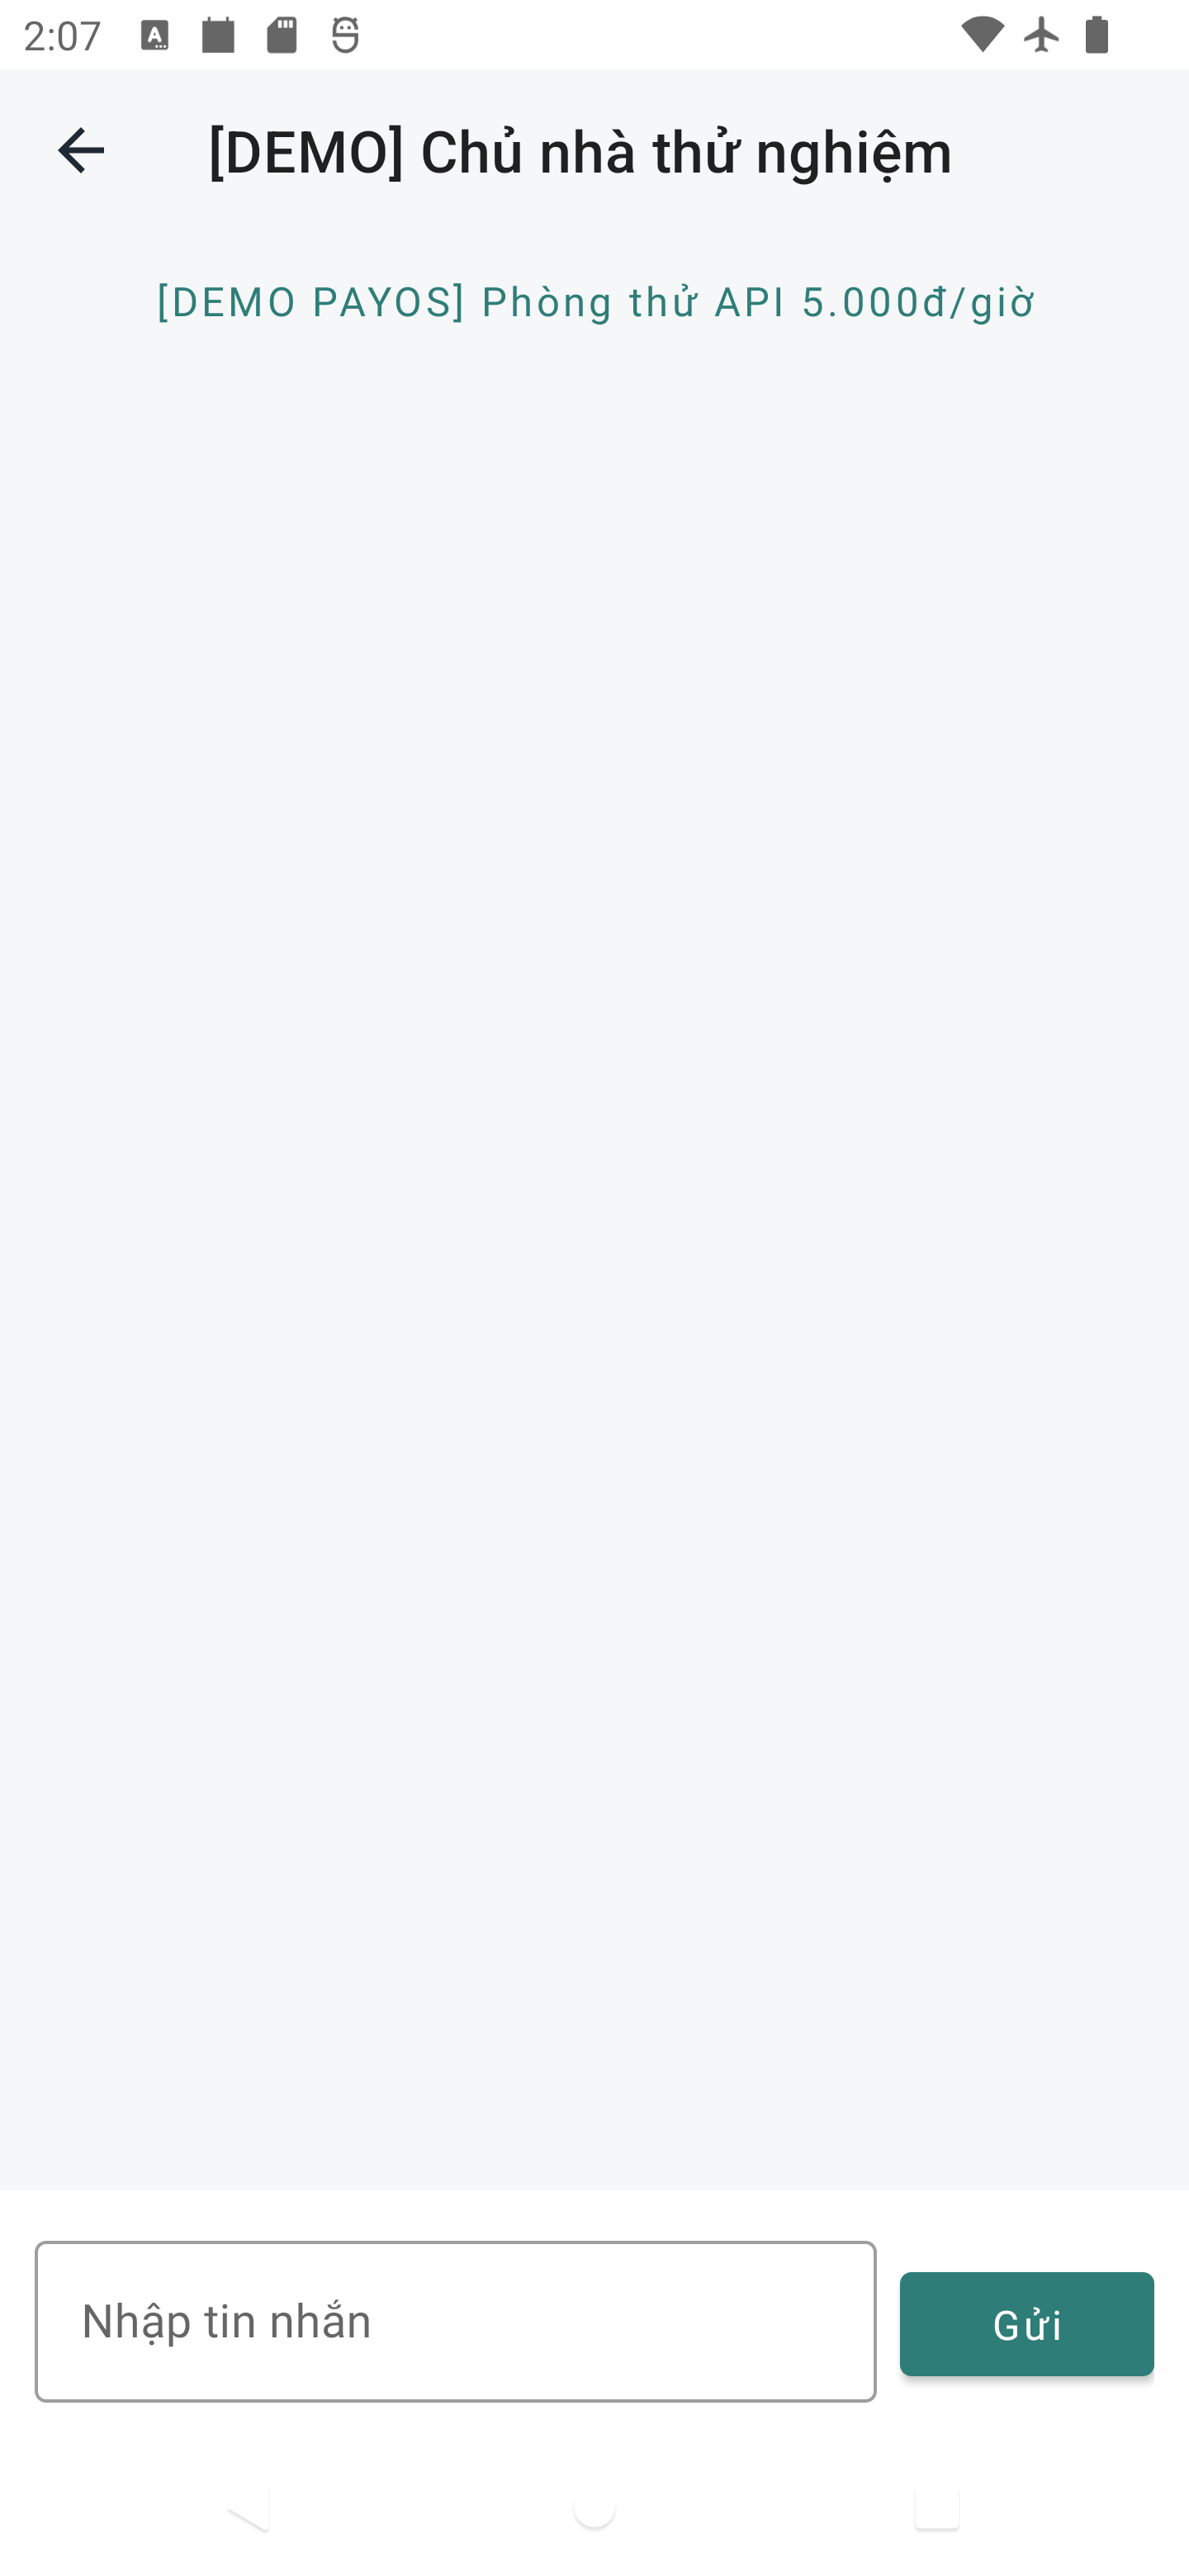
\includegraphics[width=\linewidth]{chapter5/final/conversation-detail.png}\\[-1mm]
{\small (b) Hội thoại gắn với phòng}
\end{minipage}
\caption{Danh sách hội thoại và màn trao đổi với Host}
\label{fig:actual-messages}
\end{figure}
